% Created by tikzDevice version 0.12.3.1 on 2022-05-11 22:51:47
% !TEX encoding = UTF-8 Unicode
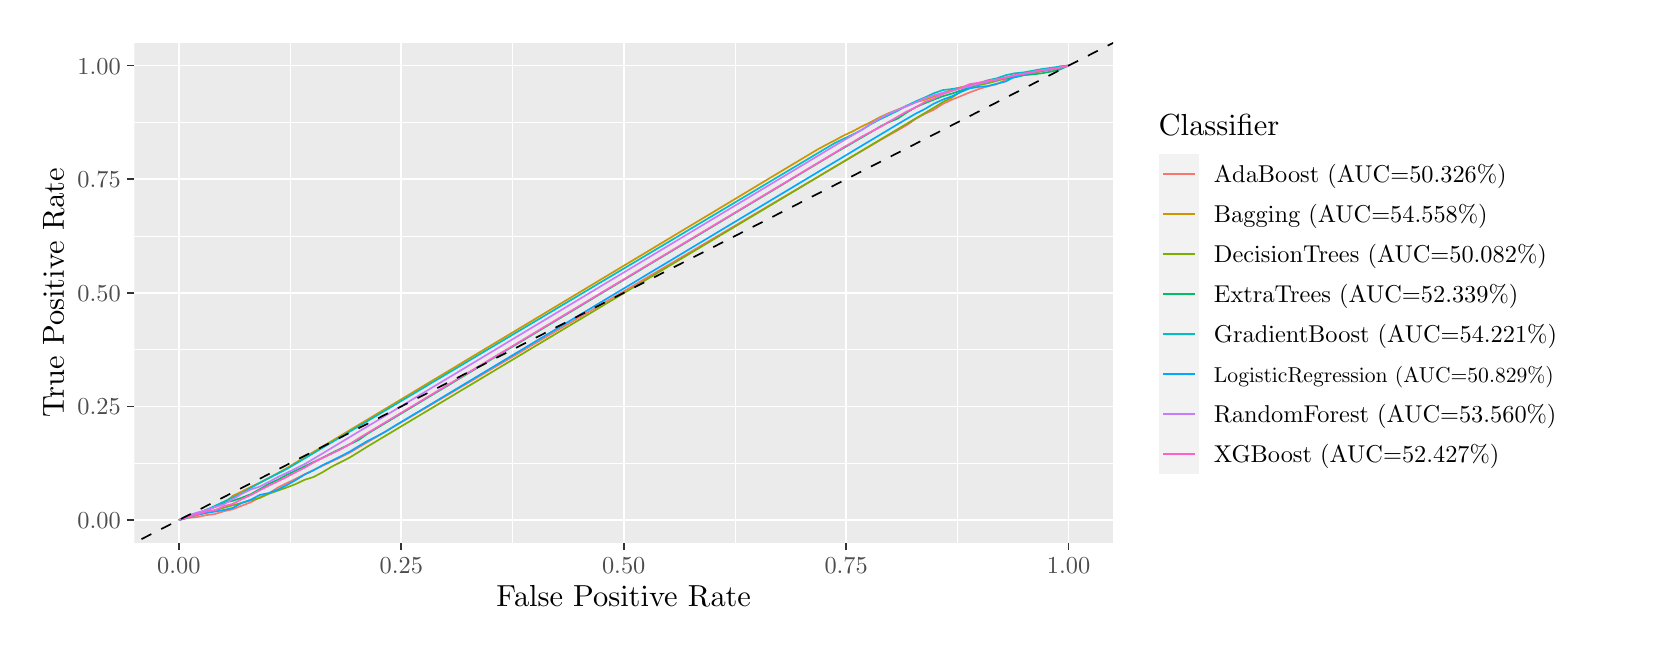
\begin{tikzpicture}[x=1pt,y=1pt]
\definecolor{fillColor}{RGB}{255,255,255}
\path[use as bounding box,fill=fillColor,fill opacity=0.00] (0,0) rectangle (578.16,216.81);
\begin{scope}
\path[clip] (  0.00,  0.00) rectangle (578.16,216.81);
\definecolor{drawColor}{RGB}{255,255,255}
\definecolor{fillColor}{RGB}{255,255,255}

\path[draw=drawColor,line width= 0.6pt,line join=round,line cap=round,fill=fillColor] (  0.00,  0.00) rectangle (578.16,216.81);
\end{scope}
\begin{scope}
\path[clip] ( 38.56, 30.69) rectangle (392.21,211.31);
\definecolor{fillColor}{gray}{0.92}

\path[fill=fillColor] ( 38.56, 30.69) rectangle (392.21,211.31);
\definecolor{drawColor}{RGB}{255,255,255}

\path[draw=drawColor,line width= 0.3pt,line join=round] ( 38.56, 59.42) --
	(392.21, 59.42);

\path[draw=drawColor,line width= 0.3pt,line join=round] ( 38.56,100.47) --
	(392.21,100.47);

\path[draw=drawColor,line width= 0.3pt,line join=round] ( 38.56,141.52) --
	(392.21,141.52);

\path[draw=drawColor,line width= 0.3pt,line join=round] ( 38.56,182.57) --
	(392.21,182.57);

\path[draw=drawColor,line width= 0.3pt,line join=round] ( 94.82, 30.69) --
	( 94.82,211.31);

\path[draw=drawColor,line width= 0.3pt,line join=round] (175.20, 30.69) --
	(175.20,211.31);

\path[draw=drawColor,line width= 0.3pt,line join=round] (255.57, 30.69) --
	(255.57,211.31);

\path[draw=drawColor,line width= 0.3pt,line join=round] (335.95, 30.69) --
	(335.95,211.31);

\path[draw=drawColor,line width= 0.6pt,line join=round] ( 38.56, 38.90) --
	(392.21, 38.90);

\path[draw=drawColor,line width= 0.6pt,line join=round] ( 38.56, 79.95) --
	(392.21, 79.95);

\path[draw=drawColor,line width= 0.6pt,line join=round] ( 38.56,121.00) --
	(392.21,121.00);

\path[draw=drawColor,line width= 0.6pt,line join=round] ( 38.56,162.05) --
	(392.21,162.05);

\path[draw=drawColor,line width= 0.6pt,line join=round] ( 38.56,203.10) --
	(392.21,203.10);

\path[draw=drawColor,line width= 0.6pt,line join=round] ( 54.63, 30.69) --
	( 54.63,211.31);

\path[draw=drawColor,line width= 0.6pt,line join=round] (135.01, 30.69) --
	(135.01,211.31);

\path[draw=drawColor,line width= 0.6pt,line join=round] (215.38, 30.69) --
	(215.38,211.31);

\path[draw=drawColor,line width= 0.6pt,line join=round] (295.76, 30.69) --
	(295.76,211.31);

\path[draw=drawColor,line width= 0.6pt,line join=round] (376.14, 30.69) --
	(376.14,211.31);
\definecolor{drawColor}{RGB}{248,118,109}

\path[draw=drawColor,line width= 0.6pt,line join=round] ( 54.63, 38.90) --
	( 57.88, 39.66) --
	( 61.13, 39.96) --
	( 64.37, 40.64) --
	( 67.62, 41.05) --
	( 70.87, 42.07) --
	( 74.12, 42.77) --
	( 77.36, 44.07) --
	( 80.61, 45.30) --
	( 83.86, 47.12) --
	( 87.11, 48.48) --
	( 90.35, 50.60) --
	( 93.60, 52.21) --
	( 96.85, 53.82) --
	(100.10, 55.45) --
	(103.34, 56.99) --
	(106.59, 58.52) --
	(109.84, 60.05) --
	(113.09, 61.59) --
	(116.33, 63.23) --
	(119.58, 65.14) --
	(122.83, 67.06) --
	(126.08, 68.97) --
	(129.32, 70.88) --
	(132.57, 72.80) --
	(135.82, 74.71) --
	(139.07, 76.62) --
	(142.31, 78.53) --
	(145.56, 80.45) --
	(148.81, 82.36) --
	(152.06, 84.27) --
	(155.30, 86.19) --
	(158.55, 88.10) --
	(161.80, 90.01) --
	(165.05, 91.92) --
	(168.29, 93.84) --
	(171.54, 95.75) --
	(174.79, 97.66) --
	(178.04, 99.58) --
	(181.28,101.49) --
	(184.53,103.40) --
	(187.78,105.31) --
	(191.03,107.23) --
	(194.27,109.14) --
	(197.52,111.05) --
	(200.77,112.97) --
	(204.02,114.88) --
	(207.26,116.79) --
	(210.51,118.70) --
	(213.76,120.62) --
	(217.01,122.53) --
	(220.26,124.44) --
	(223.50,126.36) --
	(226.75,128.27) --
	(230.00,130.18) --
	(233.25,132.09) --
	(236.49,134.01) --
	(239.74,135.92) --
	(242.99,137.83) --
	(246.24,139.75) --
	(249.48,141.66) --
	(252.73,143.57) --
	(255.98,145.48) --
	(259.23,147.40) --
	(262.47,149.31) --
	(265.72,151.22) --
	(268.97,153.14) --
	(272.22,155.05) --
	(275.46,156.96) --
	(278.71,158.87) --
	(281.96,160.79) --
	(285.21,162.70) --
	(288.45,164.61) --
	(291.70,166.53) --
	(294.95,168.44) --
	(298.20,170.35) --
	(301.44,172.26) --
	(304.69,174.18) --
	(307.94,176.09) --
	(311.19,177.93) --
	(314.43,179.74) --
	(317.68,181.61) --
	(320.93,183.87) --
	(324.18,185.67) --
	(327.42,187.14) --
	(330.67,189.26) --
	(333.92,190.76) --
	(337.17,192.08) --
	(340.41,193.44) --
	(343.66,194.62) --
	(346.91,195.64) --
	(350.16,196.38) --
	(353.40,197.98) --
	(356.65,199.08) --
	(359.90,199.70) --
	(363.15,200.39) --
	(366.39,201.07) --
	(369.64,201.56) --
	(372.89,202.80) --
	(376.14,203.10);
\definecolor{drawColor}{RGB}{205,150,0}

\path[draw=drawColor,line width= 0.6pt,line join=round] ( 54.63, 38.90) --
	( 57.88, 40.44) --
	( 61.13, 41.37) --
	( 64.37, 42.20) --
	( 67.62, 43.54) --
	( 70.87, 44.83) --
	( 74.12, 47.64) --
	( 77.36, 49.18) --
	( 80.61, 50.86) --
	( 83.86, 52.35) --
	( 87.11, 54.10) --
	( 90.35, 55.84) --
	( 93.60, 57.64) --
	( 96.85, 59.64) --
	(100.10, 61.59) --
	(103.34, 63.54) --
	(106.59, 65.49) --
	(109.84, 67.44) --
	(113.09, 69.39) --
	(116.33, 71.33) --
	(119.58, 73.28) --
	(122.83, 75.23) --
	(126.08, 77.18) --
	(129.32, 79.13) --
	(132.57, 81.08) --
	(135.82, 83.03) --
	(139.07, 84.98) --
	(142.31, 86.93) --
	(145.56, 88.88) --
	(148.81, 90.82) --
	(152.06, 92.77) --
	(155.30, 94.72) --
	(158.55, 96.67) --
	(161.80, 98.62) --
	(165.05,100.57) --
	(168.29,102.52) --
	(171.54,104.47) --
	(174.79,106.42) --
	(178.04,108.37) --
	(181.28,110.31) --
	(184.53,112.26) --
	(187.78,114.21) --
	(191.03,116.16) --
	(194.27,118.11) --
	(197.52,120.06) --
	(200.77,122.01) --
	(204.02,123.96) --
	(207.26,125.91) --
	(210.51,127.86) --
	(213.76,129.80) --
	(217.01,131.75) --
	(220.26,133.70) --
	(223.50,135.65) --
	(226.75,137.60) --
	(230.00,139.55) --
	(233.25,141.50) --
	(236.49,143.45) --
	(239.74,145.40) --
	(242.99,147.35) --
	(246.24,149.29) --
	(249.48,151.24) --
	(252.73,153.19) --
	(255.98,155.14) --
	(259.23,157.09) --
	(262.47,159.04) --
	(265.72,160.99) --
	(268.97,162.94) --
	(272.22,164.89) --
	(275.46,166.84) --
	(278.71,168.78) --
	(281.96,170.73) --
	(285.21,172.68) --
	(288.45,174.45) --
	(291.70,176.13) --
	(294.95,177.88) --
	(298.20,179.41) --
	(301.44,181.12) --
	(304.69,182.71) --
	(307.94,184.46) --
	(311.19,185.93) --
	(314.43,187.22) --
	(317.68,188.57) --
	(320.93,189.87) --
	(324.18,190.74) --
	(327.42,191.89) --
	(330.67,193.21) --
	(333.92,194.34) --
	(337.17,195.28) --
	(340.41,195.93) --
	(343.66,196.66) --
	(346.91,197.53) --
	(350.16,198.08) --
	(353.40,198.82) --
	(356.65,199.50) --
	(359.90,199.88) --
	(363.15,200.61) --
	(366.39,201.12) --
	(369.64,201.68) --
	(372.89,202.16) --
	(376.14,203.10);
\definecolor{drawColor}{RGB}{124,174,0}

\path[draw=drawColor,line width= 0.6pt,line join=round] ( 54.63, 38.90) --
	( 57.88, 39.78) --
	( 61.13, 40.67) --
	( 64.37, 41.56) --
	( 67.62, 42.44) --
	( 70.87, 43.33) --
	( 74.12, 44.22) --
	( 77.36, 45.10) --
	( 80.61, 45.99) --
	( 83.86, 46.88) --
	( 87.11, 48.38) --
	( 90.35, 49.50) --
	( 93.60, 50.65) --
	( 96.85, 51.90) --
	(100.10, 53.44) --
	(103.34, 54.45) --
	(106.59, 56.19) --
	(109.84, 58.15) --
	(113.09, 59.80) --
	(116.33, 61.45) --
	(119.58, 63.44) --
	(122.83, 65.47) --
	(126.08, 67.41) --
	(129.32, 69.35) --
	(132.57, 71.30) --
	(135.82, 73.24) --
	(139.07, 75.19) --
	(142.31, 77.13) --
	(145.56, 79.07) --
	(148.81, 81.02) --
	(152.06, 82.96) --
	(155.30, 84.91) --
	(158.55, 86.85) --
	(161.80, 88.80) --
	(165.05, 90.74) --
	(168.29, 92.68) --
	(171.54, 94.63) --
	(174.79, 96.57) --
	(178.04, 98.52) --
	(181.28,100.46) --
	(184.53,102.40) --
	(187.78,104.35) --
	(191.03,106.29) --
	(194.27,108.24) --
	(197.52,110.18) --
	(200.77,112.12) --
	(204.02,114.07) --
	(207.26,116.01) --
	(210.51,117.96) --
	(213.76,119.90) --
	(217.01,121.85) --
	(220.26,123.79) --
	(223.50,125.73) --
	(226.75,127.68) --
	(230.00,129.62) --
	(233.25,131.57) --
	(236.49,133.51) --
	(239.74,135.45) --
	(242.99,137.40) --
	(246.24,139.34) --
	(249.48,141.29) --
	(252.73,143.23) --
	(255.98,145.17) --
	(259.23,147.12) --
	(262.47,149.06) --
	(265.72,151.01) --
	(268.97,152.95) --
	(272.22,154.90) --
	(275.46,156.84) --
	(278.71,158.78) --
	(281.96,160.73) --
	(285.21,162.67) --
	(288.45,164.62) --
	(291.70,166.56) --
	(294.95,168.50) --
	(298.20,170.45) --
	(301.44,172.39) --
	(304.69,174.34) --
	(307.94,176.28) --
	(311.19,178.22) --
	(314.43,180.17) --
	(317.68,182.11) --
	(320.93,184.05) --
	(324.18,185.96) --
	(327.42,187.88) --
	(330.67,189.89) --
	(333.92,191.54) --
	(337.17,193.69) --
	(340.41,195.29) --
	(343.66,196.07) --
	(346.91,196.72) --
	(350.16,197.55) --
	(353.40,198.54) --
	(356.65,199.27) --
	(359.90,200.01) --
	(363.15,200.63) --
	(366.39,201.25) --
	(369.64,201.87) --
	(372.89,202.48) --
	(376.14,203.10);
\definecolor{drawColor}{RGB}{0,190,103}

\path[draw=drawColor,line width= 0.6pt,line join=round] ( 54.63, 38.90) --
	( 57.88, 40.01) --
	( 61.13, 41.12) --
	( 64.37, 42.54) --
	( 67.62, 43.69) --
	( 70.87, 45.22) --
	( 74.12, 45.84) --
	( 77.36, 46.96) --
	( 80.61, 48.23) --
	( 83.86, 50.04) --
	( 87.11, 51.95) --
	( 90.35, 53.43) --
	( 93.60, 55.20) --
	( 96.85, 56.74) --
	(100.10, 58.31) --
	(103.34, 59.88) --
	(106.59, 61.41) --
	(109.84, 63.11) --
	(113.09, 64.68) --
	(116.33, 66.24) --
	(119.58, 67.81) --
	(122.83, 70.09) --
	(126.08, 72.04) --
	(129.32, 73.99) --
	(132.57, 75.94) --
	(135.82, 77.89) --
	(139.07, 79.84) --
	(142.31, 81.79) --
	(145.56, 83.74) --
	(148.81, 85.69) --
	(152.06, 87.64) --
	(155.30, 89.59) --
	(158.55, 91.54) --
	(161.80, 93.49) --
	(165.05, 95.45) --
	(168.29, 97.40) --
	(171.54, 99.35) --
	(174.79,101.30) --
	(178.04,103.25) --
	(181.28,105.20) --
	(184.53,107.15) --
	(187.78,109.10) --
	(191.03,111.05) --
	(194.27,113.00) --
	(197.52,114.95) --
	(200.77,116.90) --
	(204.02,118.85) --
	(207.26,120.81) --
	(210.51,122.76) --
	(213.76,124.71) --
	(217.01,126.66) --
	(220.26,128.61) --
	(223.50,130.56) --
	(226.75,132.51) --
	(230.00,134.46) --
	(233.25,136.41) --
	(236.49,138.36) --
	(239.74,140.31) --
	(242.99,142.26) --
	(246.24,144.21) --
	(249.48,146.16) --
	(252.73,148.12) --
	(255.98,150.07) --
	(259.23,152.02) --
	(262.47,153.97) --
	(265.72,155.92) --
	(268.97,157.87) --
	(272.22,159.82) --
	(275.46,161.77) --
	(278.71,163.72) --
	(281.96,165.67) --
	(285.21,167.62) --
	(288.45,169.57) --
	(291.70,171.52) --
	(294.95,173.39) --
	(298.20,175.28) --
	(301.44,177.17) --
	(304.69,179.04) --
	(307.94,181.01) --
	(311.19,182.65) --
	(314.43,183.98) --
	(317.68,186.17) --
	(320.93,188.10) --
	(324.18,189.49) --
	(327.42,190.79) --
	(330.67,192.03) --
	(333.92,193.00) --
	(337.17,194.10) --
	(340.41,195.26) --
	(343.66,196.50) --
	(346.91,197.23) --
	(350.16,198.05) --
	(353.40,198.47) --
	(356.65,198.86) --
	(359.90,199.64) --
	(363.15,199.92) --
	(366.39,200.32) --
	(369.64,200.91) --
	(372.89,201.67) --
	(376.14,203.10);
\definecolor{drawColor}{RGB}{0,191,196}

\path[draw=drawColor,line width= 0.6pt,line join=round] ( 54.63, 38.90) --
	( 57.88, 39.73) --
	( 61.13, 41.09) --
	( 64.37, 42.45) --
	( 67.62, 43.98) --
	( 70.87, 45.53) --
	( 74.12, 47.05) --
	( 77.36, 48.57) --
	( 80.61, 50.51) --
	( 83.86, 52.34) --
	( 87.11, 54.00) --
	( 90.35, 55.65) --
	( 93.60, 57.31) --
	( 96.85, 59.23) --
	(100.10, 61.16) --
	(103.34, 63.09) --
	(106.59, 65.02) --
	(109.84, 66.95) --
	(113.09, 68.89) --
	(116.33, 70.82) --
	(119.58, 72.75) --
	(122.83, 74.68) --
	(126.08, 76.61) --
	(129.32, 78.55) --
	(132.57, 80.48) --
	(135.82, 82.41) --
	(139.07, 84.34) --
	(142.31, 86.27) --
	(145.56, 88.21) --
	(148.81, 90.14) --
	(152.06, 92.07) --
	(155.30, 94.00) --
	(158.55, 95.93) --
	(161.80, 97.87) --
	(165.05, 99.80) --
	(168.29,101.73) --
	(171.54,103.66) --
	(174.79,105.60) --
	(178.04,107.53) --
	(181.28,109.46) --
	(184.53,111.39) --
	(187.78,113.32) --
	(191.03,115.26) --
	(194.27,117.19) --
	(197.52,119.12) --
	(200.77,121.05) --
	(204.02,122.98) --
	(207.26,124.92) --
	(210.51,126.85) --
	(213.76,128.78) --
	(217.01,130.71) --
	(220.26,132.64) --
	(223.50,134.58) --
	(226.75,136.51) --
	(230.00,138.44) --
	(233.25,140.37) --
	(236.49,142.30) --
	(239.74,144.24) --
	(242.99,146.17) --
	(246.24,148.10) --
	(249.48,150.03) --
	(252.73,151.96) --
	(255.98,153.90) --
	(259.23,155.83) --
	(262.47,157.76) --
	(265.72,159.69) --
	(268.97,161.63) --
	(272.22,163.56) --
	(275.46,165.49) --
	(278.71,167.42) --
	(281.96,169.35) --
	(285.21,171.29) --
	(288.45,173.22) --
	(291.70,175.14) --
	(294.95,176.70) --
	(298.20,178.23) --
	(301.44,179.88) --
	(304.69,181.94) --
	(307.94,183.68) --
	(311.19,185.21) --
	(314.43,186.82) --
	(317.68,188.64) --
	(320.93,190.19) --
	(324.18,191.59) --
	(327.42,193.11) --
	(330.67,194.26) --
	(333.92,194.64) --
	(337.17,195.12) --
	(340.41,195.59) --
	(343.66,196.75) --
	(346.91,197.79) --
	(350.16,198.50) --
	(353.40,199.63) --
	(356.65,200.32) --
	(359.90,200.65) --
	(363.15,201.24) --
	(366.39,201.85) --
	(369.64,202.27) --
	(372.89,202.76) --
	(376.14,203.10);
\definecolor{drawColor}{RGB}{0,169,255}

\path[draw=drawColor,line width= 0.6pt,line join=round] ( 54.63, 38.90) --
	( 57.88, 40.02) --
	( 61.13, 40.83) --
	( 64.37, 41.41) --
	( 67.62, 41.95) --
	( 70.87, 42.51) --
	( 74.12, 43.27) --
	( 77.36, 45.08) --
	( 80.61, 46.23) --
	( 83.86, 47.97) --
	( 87.11, 48.64) --
	( 90.35, 49.85) --
	( 93.60, 51.50) --
	( 96.85, 53.33) --
	(100.10, 55.34) --
	(103.34, 56.88) --
	(106.59, 58.74) --
	(109.84, 60.30) --
	(113.09, 61.92) --
	(116.33, 63.59) --
	(119.58, 65.57) --
	(122.83, 67.48) --
	(126.08, 69.09) --
	(129.32, 70.85) --
	(132.57, 72.88) --
	(135.82, 74.83) --
	(139.07, 76.78) --
	(142.31, 78.72) --
	(145.56, 80.67) --
	(148.81, 82.62) --
	(152.06, 84.57) --
	(155.30, 86.51) --
	(158.55, 88.46) --
	(161.80, 90.41) --
	(165.05, 92.36) --
	(168.29, 94.31) --
	(171.54, 96.25) --
	(174.79, 98.20) --
	(178.04,100.15) --
	(181.28,102.10) --
	(184.53,104.05) --
	(187.78,105.99) --
	(191.03,107.94) --
	(194.27,109.89) --
	(197.52,111.84) --
	(200.77,113.78) --
	(204.02,115.73) --
	(207.26,117.68) --
	(210.51,119.63) --
	(213.76,121.58) --
	(217.01,123.52) --
	(220.26,125.47) --
	(223.50,127.42) --
	(226.75,129.37) --
	(230.00,131.31) --
	(233.25,133.26) --
	(236.49,135.21) --
	(239.74,137.16) --
	(242.99,139.11) --
	(246.24,141.05) --
	(249.48,143.00) --
	(252.73,144.95) --
	(255.98,146.90) --
	(259.23,148.84) --
	(262.47,150.79) --
	(265.72,152.74) --
	(268.97,154.69) --
	(272.22,156.64) --
	(275.46,158.58) --
	(278.71,160.53) --
	(281.96,162.48) --
	(285.21,164.43) --
	(288.45,166.38) --
	(291.70,168.32) --
	(294.95,170.27) --
	(298.20,172.22) --
	(301.44,174.17) --
	(304.69,176.11) --
	(307.94,178.06) --
	(311.19,180.01) --
	(314.43,181.96) --
	(317.68,183.87) --
	(320.93,185.76) --
	(324.18,187.41) --
	(327.42,189.33) --
	(330.67,190.80) --
	(333.92,192.01) --
	(337.17,193.53) --
	(340.41,194.87) --
	(343.66,195.42) --
	(346.91,195.70) --
	(350.16,196.54) --
	(353.40,197.35) --
	(356.65,199.09) --
	(359.90,199.74) --
	(363.15,200.76) --
	(366.39,201.19) --
	(369.64,201.73) --
	(372.89,202.29) --
	(376.14,203.10);
\definecolor{drawColor}{RGB}{199,124,255}

\path[draw=drawColor,line width= 0.6pt,line join=round] ( 54.63, 38.90) --
	( 57.88, 40.51) --
	( 61.13, 41.56) --
	( 64.37, 42.43) --
	( 67.62, 43.58) --
	( 70.87, 44.60) --
	( 74.12, 46.44) --
	( 77.36, 48.35) --
	( 80.61, 49.92) --
	( 83.86, 50.99) --
	( 87.11, 52.62) --
	( 90.35, 54.39) --
	( 93.60, 55.93) --
	( 96.85, 57.50) --
	(100.10, 59.12) --
	(103.34, 61.03) --
	(106.59, 62.98) --
	(109.84, 64.93) --
	(113.09, 66.89) --
	(116.33, 68.84) --
	(119.58, 70.79) --
	(122.83, 72.74) --
	(126.08, 74.69) --
	(129.32, 76.64) --
	(132.57, 78.59) --
	(135.82, 80.54) --
	(139.07, 82.49) --
	(142.31, 84.44) --
	(145.56, 86.40) --
	(148.81, 88.35) --
	(152.06, 90.30) --
	(155.30, 92.25) --
	(158.55, 94.20) --
	(161.80, 96.15) --
	(165.05, 98.10) --
	(168.29,100.05) --
	(171.54,102.00) --
	(174.79,103.96) --
	(178.04,105.91) --
	(181.28,107.86) --
	(184.53,109.81) --
	(187.78,111.76) --
	(191.03,113.71) --
	(194.27,115.66) --
	(197.52,117.61) --
	(200.77,119.56) --
	(204.02,121.52) --
	(207.26,123.47) --
	(210.51,125.42) --
	(213.76,127.37) --
	(217.01,129.32) --
	(220.26,131.27) --
	(223.50,133.22) --
	(226.75,135.17) --
	(230.00,137.12) --
	(233.25,139.08) --
	(236.49,141.03) --
	(239.74,142.98) --
	(242.99,144.93) --
	(246.24,146.88) --
	(249.48,148.83) --
	(252.73,150.78) --
	(255.98,152.73) --
	(259.23,154.68) --
	(262.47,156.64) --
	(265.72,158.59) --
	(268.97,160.54) --
	(272.22,162.49) --
	(275.46,164.44) --
	(278.71,166.39) --
	(281.96,168.34) --
	(285.21,170.29) --
	(288.45,172.24) --
	(291.70,174.20) --
	(294.95,176.13) --
	(298.20,177.98) --
	(301.44,179.94) --
	(304.69,182.10) --
	(307.94,184.06) --
	(311.19,185.73) --
	(314.43,187.13) --
	(317.68,188.41) --
	(320.93,189.81) --
	(324.18,191.28) --
	(327.42,192.39) --
	(330.67,193.31) --
	(333.92,193.96) --
	(337.17,194.87) --
	(340.41,195.60) --
	(343.66,196.53) --
	(346.91,197.27) --
	(350.16,197.97) --
	(353.40,198.85) --
	(356.65,199.54) --
	(359.90,200.20) --
	(363.15,200.80) --
	(366.39,201.44) --
	(369.64,201.86) --
	(372.89,202.25) --
	(376.14,203.10);
\definecolor{drawColor}{RGB}{255,97,204}

\path[draw=drawColor,line width= 0.6pt,line join=round] ( 54.63, 38.90) --
	( 57.88, 39.92) --
	( 61.13, 40.89) --
	( 64.37, 41.92) --
	( 67.62, 42.43) --
	( 70.87, 43.92) --
	( 74.12, 44.72) --
	( 77.36, 46.42) --
	( 80.61, 47.91) --
	( 83.86, 49.63) --
	( 87.11, 51.31) --
	( 90.35, 52.85) --
	( 93.60, 54.44) --
	( 96.85, 56.18) --
	(100.10, 57.80) --
	(103.34, 59.69) --
	(106.59, 61.33) --
	(109.84, 62.88) --
	(113.09, 64.43) --
	(116.33, 66.30) --
	(119.58, 68.42) --
	(122.83, 70.37) --
	(126.08, 72.32) --
	(129.32, 74.27) --
	(132.57, 76.22) --
	(135.82, 78.16) --
	(139.07, 80.11) --
	(142.31, 82.06) --
	(145.56, 84.01) --
	(148.81, 85.95) --
	(152.06, 87.90) --
	(155.30, 89.85) --
	(158.55, 91.80) --
	(161.80, 93.74) --
	(165.05, 95.69) --
	(168.29, 97.64) --
	(171.54, 99.59) --
	(174.79,101.53) --
	(178.04,103.48) --
	(181.28,105.43) --
	(184.53,107.38) --
	(187.78,109.33) --
	(191.03,111.27) --
	(194.27,113.22) --
	(197.52,115.17) --
	(200.77,117.12) --
	(204.02,119.06) --
	(207.26,121.01) --
	(210.51,122.96) --
	(213.76,124.91) --
	(217.01,126.85) --
	(220.26,128.80) --
	(223.50,130.75) --
	(226.75,132.70) --
	(230.00,134.64) --
	(233.25,136.59) --
	(236.49,138.54) --
	(239.74,140.49) --
	(242.99,142.44) --
	(246.24,144.38) --
	(249.48,146.33) --
	(252.73,148.28) --
	(255.98,150.23) --
	(259.23,152.17) --
	(262.47,154.12) --
	(265.72,156.07) --
	(268.97,158.02) --
	(272.22,159.96) --
	(275.46,161.91) --
	(278.71,163.86) --
	(281.96,165.81) --
	(285.21,167.75) --
	(288.45,169.70) --
	(291.70,171.65) --
	(294.95,173.67) --
	(298.20,175.48) --
	(301.44,177.46) --
	(304.69,179.16) --
	(307.94,180.83) --
	(311.19,182.78) --
	(314.43,184.68) --
	(317.68,186.54) --
	(320.93,188.00) --
	(324.18,189.98) --
	(327.42,191.17) --
	(330.67,192.77) --
	(333.92,193.95) --
	(337.17,195.01) --
	(340.41,196.42) --
	(343.66,196.93) --
	(346.91,197.58) --
	(350.16,198.11) --
	(353.40,198.68) --
	(356.65,199.70) --
	(359.90,200.08) --
	(363.15,200.71) --
	(366.39,201.39) --
	(369.64,201.71) --
	(372.89,202.44) --
	(376.14,203.10);
\definecolor{drawColor}{RGB}{0,0,0}

\path[draw=drawColor,line width= 0.6pt,dash pattern=on 4pt off 4pt ,line join=round] (-315.10,-149.94) -- (745.87,391.93);
\end{scope}
\begin{scope}
\path[clip] (  0.00,  0.00) rectangle (578.16,216.81);
\definecolor{drawColor}{gray}{0.30}

\node[text=drawColor,anchor=base east,inner sep=0pt, outer sep=0pt, scale=  0.88] at ( 33.61, 35.87) {0.00};

\node[text=drawColor,anchor=base east,inner sep=0pt, outer sep=0pt, scale=  0.88] at ( 33.61, 76.92) {0.25};

\node[text=drawColor,anchor=base east,inner sep=0pt, outer sep=0pt, scale=  0.88] at ( 33.61,117.97) {0.50};

\node[text=drawColor,anchor=base east,inner sep=0pt, outer sep=0pt, scale=  0.88] at ( 33.61,159.02) {0.75};

\node[text=drawColor,anchor=base east,inner sep=0pt, outer sep=0pt, scale=  0.88] at ( 33.61,200.07) {1.00};
\end{scope}
\begin{scope}
\path[clip] (  0.00,  0.00) rectangle (578.16,216.81);
\definecolor{drawColor}{gray}{0.20}

\path[draw=drawColor,line width= 0.6pt,line join=round] ( 35.81, 38.90) --
	( 38.56, 38.90);

\path[draw=drawColor,line width= 0.6pt,line join=round] ( 35.81, 79.95) --
	( 38.56, 79.95);

\path[draw=drawColor,line width= 0.6pt,line join=round] ( 35.81,121.00) --
	( 38.56,121.00);

\path[draw=drawColor,line width= 0.6pt,line join=round] ( 35.81,162.05) --
	( 38.56,162.05);

\path[draw=drawColor,line width= 0.6pt,line join=round] ( 35.81,203.10) --
	( 38.56,203.10);
\end{scope}
\begin{scope}
\path[clip] (  0.00,  0.00) rectangle (578.16,216.81);
\definecolor{drawColor}{gray}{0.20}

\path[draw=drawColor,line width= 0.6pt,line join=round] ( 54.63, 27.94) --
	( 54.63, 30.69);

\path[draw=drawColor,line width= 0.6pt,line join=round] (135.01, 27.94) --
	(135.01, 30.69);

\path[draw=drawColor,line width= 0.6pt,line join=round] (215.38, 27.94) --
	(215.38, 30.69);

\path[draw=drawColor,line width= 0.6pt,line join=round] (295.76, 27.94) --
	(295.76, 30.69);

\path[draw=drawColor,line width= 0.6pt,line join=round] (376.14, 27.94) --
	(376.14, 30.69);
\end{scope}
\begin{scope}
\path[clip] (  0.00,  0.00) rectangle (578.16,216.81);
\definecolor{drawColor}{gray}{0.30}

\node[text=drawColor,anchor=base,inner sep=0pt, outer sep=0pt, scale=  0.88] at ( 54.63, 19.68) {0.00};

\node[text=drawColor,anchor=base,inner sep=0pt, outer sep=0pt, scale=  0.88] at (135.01, 19.68) {0.25};

\node[text=drawColor,anchor=base,inner sep=0pt, outer sep=0pt, scale=  0.88] at (215.38, 19.68) {0.50};

\node[text=drawColor,anchor=base,inner sep=0pt, outer sep=0pt, scale=  0.88] at (295.76, 19.68) {0.75};

\node[text=drawColor,anchor=base,inner sep=0pt, outer sep=0pt, scale=  0.88] at (376.14, 19.68) {1.00};
\end{scope}
\begin{scope}
\path[clip] (  0.00,  0.00) rectangle (578.16,216.81);
\definecolor{drawColor}{RGB}{0,0,0}

\node[text=drawColor,anchor=base,inner sep=0pt, outer sep=0pt, scale=  1.10] at (215.38,  7.64) {False Positive Rate};
\end{scope}
\begin{scope}
\path[clip] (  0.00,  0.00) rectangle (578.16,216.81);
\definecolor{drawColor}{RGB}{0,0,0}

\node[text=drawColor,rotate= 90.00,anchor=base,inner sep=0pt, outer sep=0pt, scale=  1.10] at ( 13.08,121.00) {True Positive Rate};
\end{scope}
\begin{scope}
\path[clip] (  0.00,  0.00) rectangle (578.16,216.81);
\definecolor{fillColor}{RGB}{255,255,255}

\path[fill=fillColor] (403.21, 50.07) rectangle (572.66,191.92);
\end{scope}
\begin{scope}
\path[clip] (  0.00,  0.00) rectangle (578.16,216.81);
\definecolor{drawColor}{RGB}{0,0,0}

\node[text=drawColor,anchor=base west,inner sep=0pt, outer sep=0pt, scale=  1.10] at (408.71,177.78) {Classifier};
\end{scope}
\begin{scope}
\path[clip] (  0.00,  0.00) rectangle (578.16,216.81);
\definecolor{fillColor}{gray}{0.95}

\path[fill=fillColor] (408.71,156.75) rectangle (423.17,171.21);
\end{scope}
\begin{scope}
\path[clip] (  0.00,  0.00) rectangle (578.16,216.81);
\definecolor{drawColor}{RGB}{248,118,109}

\path[draw=drawColor,line width= 0.6pt,line join=round] (410.16,163.98) -- (421.72,163.98);
\end{scope}
\begin{scope}
\path[clip] (  0.00,  0.00) rectangle (578.16,216.81);
\definecolor{fillColor}{gray}{0.95}

\path[fill=fillColor] (408.71,142.30) rectangle (423.17,156.75);
\end{scope}
\begin{scope}
\path[clip] (  0.00,  0.00) rectangle (578.16,216.81);
\definecolor{drawColor}{RGB}{205,150,0}

\path[draw=drawColor,line width= 0.6pt,line join=round] (410.16,149.53) -- (421.72,149.53);
\end{scope}
\begin{scope}
\path[clip] (  0.00,  0.00) rectangle (578.16,216.81);
\definecolor{fillColor}{gray}{0.95}

\path[fill=fillColor] (408.71,127.84) rectangle (423.17,142.30);
\end{scope}
\begin{scope}
\path[clip] (  0.00,  0.00) rectangle (578.16,216.81);
\definecolor{drawColor}{RGB}{124,174,0}

\path[draw=drawColor,line width= 0.6pt,line join=round] (410.16,135.07) -- (421.72,135.07);
\end{scope}
\begin{scope}
\path[clip] (  0.00,  0.00) rectangle (578.16,216.81);
\definecolor{fillColor}{gray}{0.95}

\path[fill=fillColor] (408.71,113.39) rectangle (423.17,127.84);
\end{scope}
\begin{scope}
\path[clip] (  0.00,  0.00) rectangle (578.16,216.81);
\definecolor{drawColor}{RGB}{0,190,103}

\path[draw=drawColor,line width= 0.6pt,line join=round] (410.16,120.62) -- (421.72,120.62);
\end{scope}
\begin{scope}
\path[clip] (  0.00,  0.00) rectangle (578.16,216.81);
\definecolor{fillColor}{gray}{0.95}

\path[fill=fillColor] (408.71, 98.94) rectangle (423.17,113.39);
\end{scope}
\begin{scope}
\path[clip] (  0.00,  0.00) rectangle (578.16,216.81);
\definecolor{drawColor}{RGB}{0,191,196}

\path[draw=drawColor,line width= 0.6pt,line join=round] (410.16,106.16) -- (421.72,106.16);
\end{scope}
\begin{scope}
\path[clip] (  0.00,  0.00) rectangle (578.16,216.81);
\definecolor{fillColor}{gray}{0.95}

\path[fill=fillColor] (408.71, 84.48) rectangle (423.17, 98.94);
\end{scope}
\begin{scope}
\path[clip] (  0.00,  0.00) rectangle (578.16,216.81);
\definecolor{drawColor}{RGB}{0,169,255}

\path[draw=drawColor,line width= 0.6pt,line join=round] (410.16, 91.71) -- (421.72, 91.71);
\end{scope}
\begin{scope}
\path[clip] (  0.00,  0.00) rectangle (578.16,216.81);
\definecolor{fillColor}{gray}{0.95}

\path[fill=fillColor] (408.71, 70.03) rectangle (423.17, 84.48);
\end{scope}
\begin{scope}
\path[clip] (  0.00,  0.00) rectangle (578.16,216.81);
\definecolor{drawColor}{RGB}{199,124,255}

\path[draw=drawColor,line width= 0.6pt,line join=round] (410.16, 77.26) -- (421.72, 77.26);
\end{scope}
\begin{scope}
\path[clip] (  0.00,  0.00) rectangle (578.16,216.81);
\definecolor{fillColor}{gray}{0.95}

\path[fill=fillColor] (408.71, 55.57) rectangle (423.17, 70.03);
\end{scope}
\begin{scope}
\path[clip] (  0.00,  0.00) rectangle (578.16,216.81);
\definecolor{drawColor}{RGB}{255,97,204}

\path[draw=drawColor,line width= 0.6pt,line join=round] (410.16, 62.80) -- (421.72, 62.80);
\end{scope}
\begin{scope}
\path[clip] (  0.00,  0.00) rectangle (578.16,216.81);
\definecolor{drawColor}{RGB}{0,0,0}

\node[text=drawColor,anchor=base west,inner sep=0pt, outer sep=0pt, scale=  0.88] at (428.67,160.95) {AdaBoost (AUC=50.326\%)};
\end{scope}
\begin{scope}
\path[clip] (  0.00,  0.00) rectangle (578.16,216.81);
\definecolor{drawColor}{RGB}{0,0,0}

\node[text=drawColor,anchor=base west,inner sep=0pt, outer sep=0pt, scale=  0.88] at (428.67,146.50) {Bagging (AUC=54.558\%)};
\end{scope}
\begin{scope}
\path[clip] (  0.00,  0.00) rectangle (578.16,216.81);
\definecolor{drawColor}{RGB}{0,0,0}

\node[text=drawColor,anchor=base west,inner sep=0pt, outer sep=0pt, scale=  0.88] at (428.67,132.04) {DecisionTrees (AUC=50.082\%)};
\end{scope}
\begin{scope}
\path[clip] (  0.00,  0.00) rectangle (578.16,216.81);
\definecolor{drawColor}{RGB}{0,0,0}

\node[text=drawColor,anchor=base west,inner sep=0pt, outer sep=0pt, scale=  0.88] at (428.67,117.59) {ExtraTrees (AUC=52.339\%)};
\end{scope}
\begin{scope}
\path[clip] (  0.00,  0.00) rectangle (578.16,216.81);
\definecolor{drawColor}{RGB}{0,0,0}

\node[text=drawColor,anchor=base west,inner sep=0pt, outer sep=0pt, scale=  0.88] at (428.67,103.13) {GradientBoost (AUC=54.221\%)};
\end{scope}
\begin{scope}
\path[clip] (  0.00,  0.00) rectangle (578.16,216.81);
\definecolor{drawColor}{RGB}{0,0,0}

\node[text=drawColor,anchor=base west,inner sep=0pt, outer sep=0pt, scale=  0.78] at (428.67, 88.68) {LogisticRegression (AUC=50.829\%)};
\end{scope}
\begin{scope}
\path[clip] (  0.00,  0.00) rectangle (578.16,216.81);
\definecolor{drawColor}{RGB}{0,0,0}

\node[text=drawColor,anchor=base west,inner sep=0pt, outer sep=0pt, scale=  0.88] at (428.67, 74.23) {RandomForest (AUC=53.560\%)};
\end{scope}
\begin{scope}
\path[clip] (  0.00,  0.00) rectangle (578.16,216.81);
\definecolor{drawColor}{RGB}{0,0,0}

\node[text=drawColor,anchor=base west,inner sep=0pt, outer sep=0pt, scale=  0.88] at (428.67, 59.77) {XGBoost (AUC=52.427\%)};
\end{scope}
\end{tikzpicture}
